\chapter{Deployment}
\label{sec:deployment}

This chapter shows different deployment and usage options for the Henshin Web editor. The options are evaluated and the best one is selected. Finally, the implementation of the deployment is described.

\section{GLSP Integration Options}
\label{sec:integration-options}
A \ac{glsp} editor can be deployed and used in production in various ways. \ac{glsp} provides platform integrations for the Eclipse Desktop IDE, Eclipse Theia, \ac{vscode}, and as a standalone web application. Each integration brings different integration possibilities, deployment, and usage options for the editor. \cite{glsp-doc} The main considerations for the deployment and usage are:
  \begin{itemize}
    \item The user should need as few dependencies as possible. Dependencies are a browser runtime, an \acs{ide} to install, or an extension to install.
    \item The app should be easy to access. Possible barriers are the creation of an account or the installation of dependencies.
    \item Using a self-hosted server or a cloud service. With a self-hosted server, the user has full access of local files to open and edit. With a cloud service, the user has to upload and download files to the server.
  \end{itemize}
  
  To use \ac{glsp} as a standalone web application, a dependency injection container with the custom \ac{glsp} client is added to a TypeScript browser application. Like that the editor of a certain file as a data source can be displayed. When the app is hosted, no other dependency than a browser runtime is needed to use the standalone diagram editor. \cite{glsp-client-repo} This option provides the most flexibility, as it can be used in any web application, but also requires the most effort to implement, when developing a complete editor. All features, like file management, window management, or other features a \acs{ide} brings, need to be implemented by the developer. \cite{glsp-client-repo} For our use case, the standalone web application is not an option, as these additional features are needed. 

  The other \ac{glsp} integrations are \acs{ide} integrations and therefore provide many features out of the box. For the Eclipse \acs{ide} integration, Eclipse has to be installed, and the \ac{glsp} plugin has to be added to the Eclipse installation. The plugin can be installed from the Eclipse Marketplace or manually by downloading the plugin jar file. \cite{eclipse-doc} The \ac{vscode} integration also provides this option. The \acs{ide} can be installed and the \ac{glsp} editor can be added as an extension. The extension can be installed from the Marketplace or manually using a \textit{.vsix} file. \cite{vscode-doc} The \ac{glsp} \ac{vscode} integration can provide a \textit{.vsix} file. \cite{glsp-repo} \ac{vscode} is the most used \acs{ide}. 73.6\% of developers use \ac{vscode} due to the survey of \citeauthor{stackoverflow2024survey} In \citeyear{stackoverflow2024survey} \cite{stackoverflow2024survey}. An advantage to Eclipse is that \ac{vscode} provides a browser version, which brings the same capabilites as the desktop \acs{ide}. \cite{vscode-doc} So this integration provides the advantage that no \acs{ide} has to be installed to be able to use Henshin Web. The user can open \ac{vscode}, add the extension, and directly open a metamodel, rule, or instance model file and start editing. 

  The Eclipse Theia \acs{ide} is not as widely popular as \ac{vscode} \cite{stackoverflow2024survey}, but its focus is not to provide a ready \acs{ide} but to provide tools to create custom \acsp{ide}. The Eclipse Theia project is part of the Eclipse Foundation and is used as a basis to create your own \acsp{ide} based on web technologies. \cite{theia-doc} They provide the Theia IDE that acts as a template editor and can be downloaded and used on all common operating systems or used in as a web editor in the browser. Due to the focus on providing a framework to build custom \acsp{ide}, Theia provides more options to use extensions and plugins to extend the functionality. You can see the options and their architectural integration into Theia in figure \ref{fig:theia-extensions}.
  \begin{itemize}
    \item \textbf{\ac{vscode} extensions} Theia provides the \ac{vscode} extension \acs{api}, so that existing \ac{vscode} extensions can be used in Theia. They only interact with the \acs{api} and therefore can be installed at runtime.
    \item \textbf{Theia plugins} are working like \ac{vscode} extensions. They interact with the Theia plugin \acs{api} and can also access the \ac{vscode} extension \acs{api}. They can access some Theia specific features, that \ac{vscode} extensions cannot access, like directly contributing to the frontend. They can also be installed at runtime, or be pre-installed at compile time.
    \item \textbf{Headless plugins} are also working like \ac{vscode} extensions. They can also be installed at runtime and can access custom extended Theia backend services.
    \item \textbf{Theia extensions} are the core architecture parts of Theia. Theia is fully built using Theia extensions in a modular way. The template Theia \acs{ide} contains Theia extensions, including the core. Custom Theia extensions can be developed and added to Theia with full access to all Theia functionality via dependency injection. They need to be installed at compile time. \cite{theia-doc}
  \end{itemize}

  The \ac{glsp} Theia integration is creating a Theia extension, that is packed into a custom Theia \acs{ide}. It is also possible to use the \ac{glsp} \ac{vscode} integration that provides a \ac{vscode} extension, that can also be added to a Theia \acs{ide} at runtime. \cite{glsp-repo} The option to use the diagram editor in the browser makes the \ac{glsp} Eclipse integration not interesting for Hensin Web. \ac{vscode} has the advantage of popularity and simplicity to use the editor without any registration or installation. Eclipse Theia has the advantage of modularity and further extensibility. Further features can be added in the future to provide a web-based environment for \ac{mde}. Theia also provides different ways to deploy a Theia \acs{ide}.   These considerations show that the Theia integration is the best option for deploying the Henshin Web editor. Theia combines the advantages of browser-based access, modularity, and extensibility.

  \begin{figure}[h]
    \centering
    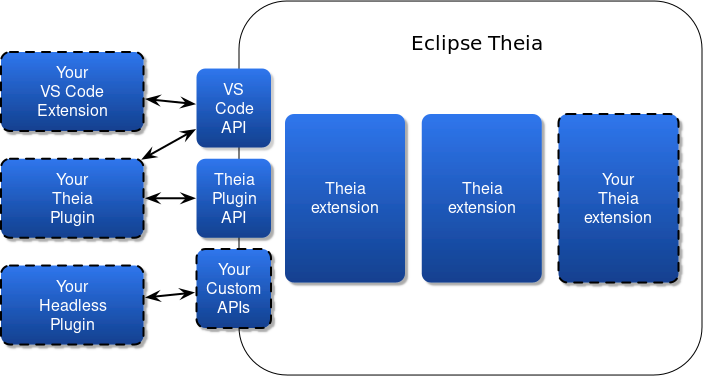
\includegraphics[width=0.7\textwidth]{theia-extension}
    \caption{Theia high level extensions and plugins architecture. Image obtained from \cite{theia-doc}}
    \label{fig:theia-extensions}
  \end{figure}


  \section{Deployment Options and Evaluation}
  \label{sec:deployment-evaluation}

  
  There are different options to provide a \ac{glsp} Theia application. The Theia editor, consisting of the TypeScript client and the Java server, can be hosted in the cloud and accessed via a web browser. The Eclipse Foundation provides the Theia Cloud project \cite{theia-cloud-doc} to deploy Theia based products on Kubernetes clusters \cite{kubernetes}. Theia Cloud introduces three custom Kubernetes resource types. \textit{App Definitions} contain all necessary information about the Theia based product. \textit{Workspaces} define persistent storage solutions, where metamodel, rule, or instance model files can be stored for each user. \textit{Sessions} are acting as a runtime representaions. Theia Cloud includes components like a landing page, authentication, authorization, a cloud monitor, and a cloud operator, that deploys sessions and manages workspaces. You can see the different components and their interactions in figure \ref{fig:theia-cloud-components}. The service provides two preconfigured configurations for quickly trying out Theia Cloud on a cluster. \cite{theia-cloud-doc}

  \begin{figure}[h]
    \centering
    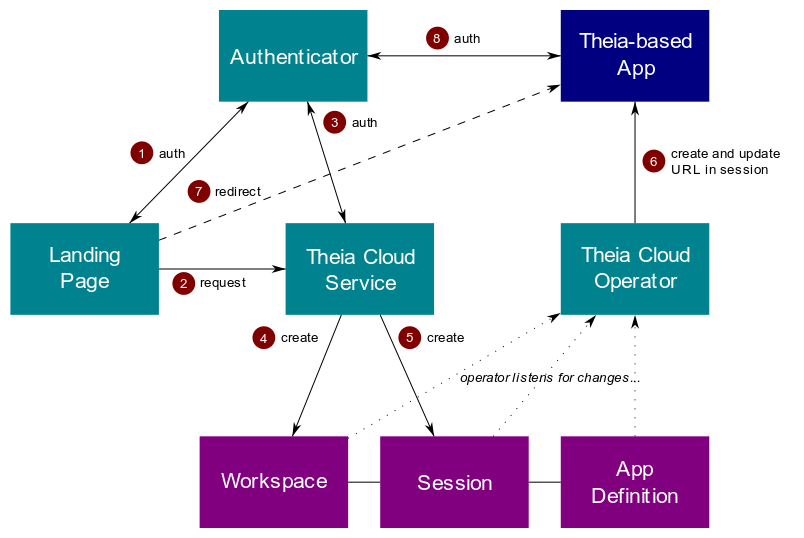
\includegraphics[width=0.7\textwidth]{theia-cloud-components.png}
    \caption{Interaction between Theia Cloud components. Image obtained from \cite{theia-cloud-doc}}
    \label{fig:theia-cloud-components}
  \end{figure}

  Because of the limited file access of the browser, the user has to upload and download all files to the server to use them. To be able to access the local file system of the user directly, the server needs to be hosted locally. For that, \ac{glsp} Theia application can be hosted in a Docker container. \cite{docker} The Docker container can contain the Java server and the TypeScript client, that are started together. The user can then access the editor via a web browser. On a machine with a Docker environment, this solution can be started locally in an easy way and has the access to the file system. The Docker container can also be used to deploy the application on a server so that it can be accessed by multiple users. The single Docker container solution doesn't provide as much scalability as using a cluster with Theia Cloud.

  The \ac{glsp} Theia application can also be used as a desktop application. Theia uses Electron \cite{electron-repo} to bundle the application into a desktop application, that can be installed via an installer. This approach also provides access to the local file system, since the electron application works like a self-hosted web application, and therefore the \ac{glsp} Java server is started locally. All in all, the \ac{glsp} Theia integration provides all different options to use the Henshin Web editor. Further clients can always be added later if needed.

  \begin{table}[h]
  \centering
  \caption{Comparison of GLSP Theia deployment options}
  \label{tab:deployment-comparison}
  \resizebox{\textwidth}{!}{
    \begin{tabular}{|l|p{3.2cm}|p{3.2cm}|p{3.2cm}|p{3.2cm}|}
      \hline
      \textbf{Option} & \textbf{Self-hosted Container} & \textbf{Cloud Hosted Container} & \textbf{Theia Cloud} & \textbf{Desktop (Electron)} \\
      \hline
      \textbf{Installation Effort} & Local Docker Setup required & None (access via browser) & None (creating an account) & Installing over a standard installer \\
      \hline
      \textbf{Dependencies} & Docker runtime, web browser & Web browser only & Web browser only & Application installer \\
      \hline
      \textbf{Multi-user Support} & Single user & Multi-user possible but no shared editor & Built-in shared workspaces, but no shared editor & Single user per installation \\
      \hline
      \textbf{Hosting Requirements} & Local & Cloud service (Container hosting) & Kubernetes cluster & Local machine \\
      \hline
      \textbf{Cross-platform} & Yes (via browser) & Yes (via browser) & Yes (via browser) & Platform-specific builds \\
      \hline
      \textbf{Offline Usage} & Yes & No & No & Yes \\
      \hline
      \textbf{File System Access} & Full local access & Upload/download required & Upload/download required & Full local access \\
      \hline
      \textbf{Costs} & No Costs & Cloud server costs & Cost of Google Cloud Kubernetes cluster & No Costs (maybe provisioning of installer) \\
      \hline
    \end{tabular}
  }
\end{table}

  In table \ref{tab:deployment-comparison} the different deployment options are listed. Each pair of options is similar.The self-hosted Docker and Desktop Electron bring no costs to provide the application, can be used offline and provide full local file access. Here the Desktop option is easier to install and use, as no external dependencies need to be installed before. And even thought it doesn't use the browser, it is based on web technologies. The other two similar options are host a container in the cloud and using Theia Cloud. A cloud hosted container would be a self implemented and configured solution. That would bring more flexibility, but also more effort to implement and maintain. Especially when the user management and workspace management should be implemented. Theia Cloud on the other hand provides these features out of the box. Both options bring costs for hosting the server and need an internet connection to be used. They also don't provide access to the local file system, as they are not self-hosted. Since Theia Cloud also leaves configuration options open and it is made for hosting Theia based products, it is the better option to host Henshin Web in the cloud.
  Now the decision is between the Electron desktop application and Theia Cloud. The desktop application has the advantages, that it can be used offline and provides full access to the local file system. This would be no bid difference to use Henshin in the Eclipse IDE. Theia Cloud on the other hand provides the advantage of easy access via a web browser without any installation. It also provides the possibility to use Henshin Web on different devices, like tablets or smartphones. Therefore Theia Cloud is the best fitting option to deploy Henshin Web.
  
 \section{Deployment Implementation}
  \label{sec:deployment-implementation}

  This chapter describes the implementation of the deployment of Henshin Web using Theia Cloud. Theia Cloud provides two different deployment options to host the application on. It is possible to host the application on a Kubernetes cluster in the Google Cloud using \ac{gke} or on a local Kubernetes cluster using minicube. The following implementation shows the deployment using \ac{gke}. The implementation using minicube is similar, only the terraform code and the prerequisites of the local machine are different.

  \subsection{Docker Container Architecture}
  \label{subsec:docker-architecture}

  The first thing that needs to be done is to create a docker image of the application. The docker image contains the Java server and the TypeScript client. The resulting docker file is shown in listing \ref{lst:dockerfile}. The Dockerfile implements a multi-stage build approach. This approach separates the build environment from the runtime environment, resulting in smaller and more secure production containers. The build process consists of three distinct stages, each serving a specific purpose in the containerization pipeline. This separation allows for parallel execution of backend and frontend builds, improving overall build performance.

  The first stage, labeled as \textit{build}, establishes the development environment using a Debian Bullseye image with Node.js preinstalled. This stage installs all necessary dependencies for building both the Java backend and TypeScript frontend components. The environment includes Maven for Java compilation, OpenJDK 17 for runtime compatibility, and various system libraries required by Theia. The second stage, \textit{backend}, focuses on compiling the \ac{glsp} Java server. It copies the server source code and uses Maven to clean, compile, and verify the Java components. The Maven settings file is copied to handle GitLab authentication for private repositories, ensuring that all dependencies can be resolved during the build process. The third stage, \textit{frontend}, handles the compilation of all Theia components and plugins. The Yarn autoclean feature is configured to remove unnecessary files like TypeScript sources and test files from the final image, reducing the container size. The final production stage uses a slim Debian image to minimize the attack surface and container size. It installs only the runtime dependencies necessary for Theia operation, including Java runtime, system libraries, and development tools. A non-root user with ID 200 is created, following Theia Cloud standards for user management. The home directory is properly configured with appropriate permissions for file operations. The container exposes port 3000 for web access and configures the entry point to start the Theia backend server with specific parameters for workspace management and plugin loading.

 \subsection{Terraform Configuration}
\label{subsec:terraform-configuration}

When the docker image is built, it can be used to deploy the application on \ac{gke} to make it accessible via the internet for everyone. Theia Cloud provides a modular terraform \cite{terraform-repo} configuration to deploy the Kubernetes cluster to the Google Cloud. This \ac{iac} approach provides the advantage that the infrastructure can be defined as code and therefore can be easily adapted, versioned, and reused.

The Terraform configuration follows a modular architecture with three main components: cluster creation, Helm chart deployment, and Keycloak \cite{keycloak-repo} authentication setup. The main configuration file orchestrates the deployment by calling specialized modules that handle specific infrastructure concerns.

The cluster creation module provisions a production-ready \ac{gke} cluster with auto-scaling node pools. The configuration removes the default node pool to enable custom machine types (\texttt{e2-standard-2}) and scaling parameters (1-2 nodes), providing cost optimization while ensuring adequate resources:

\begin{lstlisting}[language=hcl, caption=GKE Cluster Configuration]
resource "google_container_cluster" "primary" {
  name                     = var.cluster_name
  location                 = var.location
  remove_default_node_pool = true
  initial_node_count       = 1
  deletion_protection      = false
}
\end{lstlisting}

Network connectivity is established through a reserved static IP address that supports both custom domains and automatic DNS resolution via sslip.io. The configuration integrates multiple providers (Google Cloud, Helm, Kubectl, Keycloak \cite{keycloak-repo}) with dynamic authentication using cluster credentials obtained from the GKE module.

The Helm module manages the deployment of essential Kubernetes applications including NGINX Ingress Controller, Cert-Manager for SSL certificates, Keycloak \cite{keycloak-repo} for authentication, PostgreSQL database, and the Theia Cloud application components. Variable management separates configuration from sensitive data, with security-sensitive variables marked appropriately:

\begin{lstlisting}[language=hcl, caption=Variable Configuration]
variable "keycloak_admin_password" {
  description = "Keycloak Admin Password"
  type        = string
  sensitive   = true
}

variable "theia_docker_image" {
  description = "Docker image for your Theia application"
  type        = string
  default     = "gcr.io/henshin-web/henshin-web-model-transformation:latest"
}
\end{lstlisting}

% \subsection{Deployment Execution}
% \label{subsec:deployment-execution}

% The target for the deployment is that it executes automatically in the CI\CD pipeline of the project. Due to restrictions in the used Gitlab instance, the deployment have to be executed manually. Without image-restrictions for the build pipeline, the automatic deployment could be implemented.

% To deploy the project, the prerequisites are that the Google Cloud SDK, Docker, and Terraform are installed on the local machine. The Google Cloud SDK needs to be authenticated with a Google account that has permissions to create and manage \ac{gke} clusters. Docker needs to be installed and running to build the docker image. Terraform needs to be installed to execute the deployment configuration.

% To make the manual deployment easy, a PowerShell script is created that automates the deployment steps. The script first checks if all prerequisites are installed and configured. Then it builds the docker image and pushes it to the Google Container Registry. Finally, it initializes Terraform, plans the deployment, and applies the configuration to deploy the application on \ac{gke}. The script can be found in the project repository \cite{henshin-web-repo}.

\subsection{Deployment Execution}
\label{subsec:deployment-execution}

The deployment of the Henshin Web application follows a systematic process that combines containerization, cloud infrastructure provisioning, and configuration management. The deployment workflow is automated through PowerShell scripts that orchestrate the entire process from local development to production deployment on Google Cloud Platform.

Before executing the deployment, several prerequisites must be satisfied:

\begin{itemize}
    \item Google Cloud Platform account with billing enabled
    \item Google Cloud SDK (gcloud) installed and authenticated
    \item Docker Desktop or Docker Engine installed
    \item Terraform CLI installed (version >= 1.4.0)
    \item Access to the project's Google Container Registry
\end{itemize}

The first step involves building the Docker container and pushing it to Google Container Registry. This process is automated through the \texttt{build-and-push.ps1} script:

\begin{lstlisting}[language=powershell, caption=Container Build Process]
docker build -t "henshin-web-model-transformation:latest" .

$FullImageName = "gcr.io/henshin-web/henshin-web-model-transformation:latest"

docker tag "henshin-web-model-transformation:latest" $FullImageName
docker push $FullImageName
\end{lstlisting}

Once the container image is available in the registry, the infrastructure deployment is executed through the \texttt{deploy.ps1} script. This script starts the creation of the resources in the Google Cloud using Terraform:

\begin{lstlisting}[language=powershell, caption=Infrastructure Deployment]
Set-Location "$PSScriptRoot\..\terraform\configurations\henshin-web-app"

terraform init

$env:GOOGLE_OAUTH_ACCESS_TOKEN = (gcloud auth print-access-token)
terraform apply
\end{lstlisting}

The deployment script automatically handles authentication by obtaining fresh OAuth tokens from the gcloud CLI. This ensures that Terraform has the necessary permissions to create and manage Google Cloud resources without requiring manual token management.

The Terraform configuration executes the deployment in a specific sequence to ensure proper dependency resolution:

\begin{enumerate}
    \item \textbf{GKE Cluster Creation}: Provisions the Kubernetes cluster with auto-scaling node pools
    \item \textbf{Network Configuration}: Reserves static IP addresses and configures ingress rules
    \item \textbf{Core Services Deployment}: Installs NGINX Ingress Controller and Cert-Manager
    \item \textbf{Database Setup}: Deploys PostgreSQL for Keycloak authentication services
    \item \textbf{Authentication Configuration}: Installs and configures Keycloak with realm settings
    \item \textbf{Application Deployment}: Deploys the Henshin Web application and landing page
    \item \textbf{SSL Certificate Provisioning}: Automatically obtains Let's Encrypt certificates
\end{enumerate}

The deployment process uses environment-specific configuration through the \texttt{terraform.tfvars} file, which contains:

\begin{itemize}
    \item Project identification and resource naming conventions
    \item Container image references with specific tags
    \item Authentication credentials for Keycloak and database services
    \item Regional deployment settings and cluster specifications
\end{itemize}

Because this includes sensitive configuration values, they are managed separately from the codebase to maintain security best practices while enabling automated deployment workflows.

Upon successful completion, the deployment script provides the application URL, typically in the format \texttt{https://<static-ip>.sslip.io}, where the application becomes immediately accessible. The automated SSL certificate provisioning through Let's Encrypt ensures secure HTTPS connectivity without manual certificate management.

The deployment can be reversed using the \texttt{destroy.ps1} script, which safely removes all provisioned resources while preserving any persistent data that needs to be retained for future deployments.